\chapter{Sprint 0 : Initialisation et Configuration}
\label{chap:sprint-0}

\section{Introduction}

Le Sprint 0 constitute la phase preparatoire du projet, destinee a mettre en place l'environnement de developpement, a configurer l'infrastructure, a concevoir l'architecture initiale et a etablir les conventions de developpement. Ce sprint ne produit pas de fonctionnalites directement operationnelles mais pose les bases techniques et organisationnelles necesaires pour les sprints suivants.

Le Sprint 0 s'est deroule sur deux semaines et a permis de :
\begin{itemize}
    \item etablir l'architecture multi-service de la plateforme,
    \item configurer l'environnement de developpement local,
    \item initialiser les repositories Git et la structure du projet,
    \item concevoir les bases de donnees,
    \item mettre en place la conteneurisation Docker,
    \item configurer les services externes (n8n, Gemini API).
\end{itemize}

\section{Objectifs du Sprint 0}

Les objectifs principaux du Sprint 0 etaient :

\begin{enumerate}
    \item \textbf{Definir l'architecture multi-service} : concevoir une architecture modulaire exploitant les forces de chaque technologie,
    
    \item \textbf{Configurer l'infrastructure Docker} : mettre en place des conteneurs pour PostgreSQL, n8n et les services principaux,
    
    \item \textbf{Initialiser la base de donnees} : creer le schema relationnels et les tables de base,
    
    \item \textbf{Mettre en place le backend Spring Boot} : initialiser le projet Maven, configurer les dependances et les configurations,
    
    \item \textbf{Initialiser le frontend React} : creer la structure du projet React avec routing de base,
    
    \item \textbf{Creer le service Python} : initialiser le projet FastAPI pour l'extraction de documents,
    
    \item \textbf{Documenter l'environnement} : produire un guide de demarrage pour l'equipe de developpement,
    
    \item \textbf{Etablir les conventions de developpement} : definir les standards de code, de nommage et de structure.
\end{enumerate}

\section{Architecture Initiale Concue}

\subsection{Vue d'ensemble}

L'architecture retenue suit un pattern microservices avec orchestration de workflows. Chaque service possede une responsabilite bien definie :

\begin{figure}[!ht]
\centering
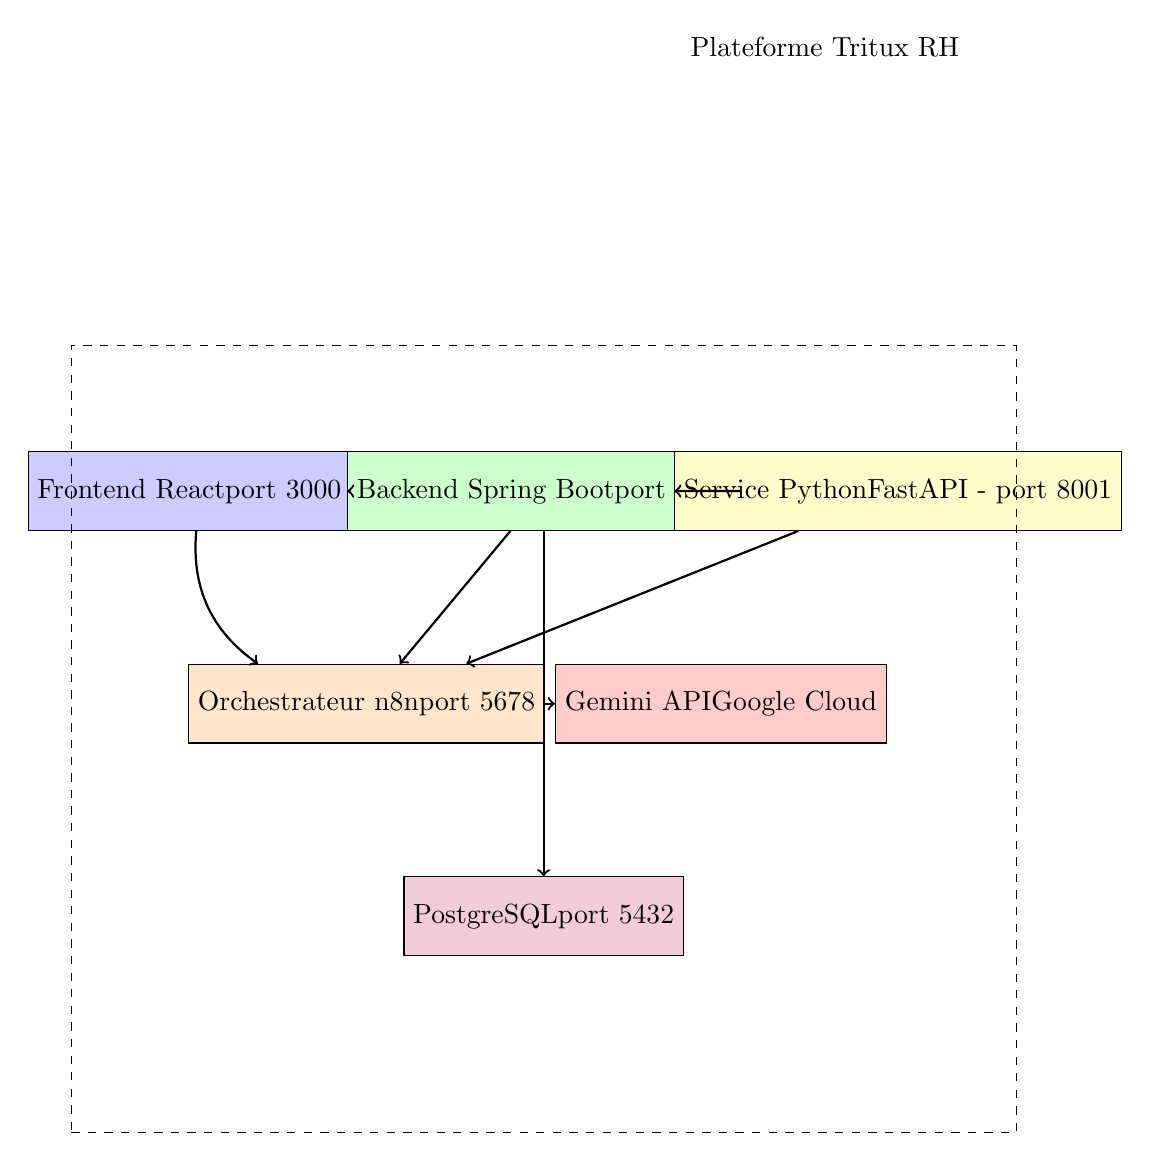
\begin{tikzpicture}[scale=0.9]
    % Frontend
    \node[draw, rectangle, minimum width=3cm, minimum height=1cm, fill=blue!20] (frontend) at (0,8) {Frontend React\\port 3000};
    
    % Backend
    \node[draw, rectangle, minimum width=3cm, minimum height=1cm, fill=green!20] (backend) at (5,8) {Backend Spring Boot\\port 9091};
    
    % Python Service
    \node[draw, rectangle, minimum width=3cm, minimum height=1cm, fill=yellow!20] (python) at (10,8) {Service Python\\FastAPI - port 8001};
    
    % Orchestrateur
    \node[draw, rectangle, minimum width=3cm, minimum height=1cm, fill=orange!20] (n8n) at (2.5,5) {Orchestrateur n8n\\port 5678};
    
    % Gemini API
    \node[draw, rectangle, minimum width=3cm, minimum height=1cm, fill=red!20] (gemini) at (7.5,5) {Gemini API\\Google Cloud};
    
    % Database
    \node[draw, rectangle, minimum width=3cm, minimum height=1cm, fill=purple!20] (db) at (5,2) {PostgreSQL\\port 5432};
    
    % Connections
    \draw[->, thick] (frontend) -- (backend);
    \draw[->, thick] (backend) -- (python);
    \draw[->, thick] (backend) -- (n8n);
    \draw[->, thick] (python) -- (n8n);
    \draw[->, thick] (n8n) -- (gemini);
    \draw[->, thick] (backend) -- (db);
    \draw[->, thick] (frontend) to[bend right] (n8n);
    
    \node[draw, rectangle, dashed, minimum width=12cm, minimum height=10cm] at (5,4.5) {};
    \node[anchor=south east, dashed] at (11,14) {Plateforme Tritux RH};
\end{tikzpicture}
\caption{Architecture multi-service de la plateforme}
\label{fig:architecture-sprint0}
\end{figure}

\subsection{Decomposition des services}

\subsubsection{Frontend React (port 3000)}

Le frontend est une application React 18 mettant en œuvre une \acrfull{ui} reactive et ergonomique. Ses caracteristiques principales :

\begin{itemize}
    \item \textbf{Framework} : React 18.3 avec React Router 6.23 pour le routing,
    
    \item \textbf{Styling} : Tailwind CSS 3.4 pour une coherence visuelle,
    
    \item \textbf{HTTP Client} : Axios 1.7 pour les appels API REST,
    
    \item \textbf{Modules} : Dashboard, Profiles, Templates, Transformation, JobOffers, Chat,
    
    \item \textbf{Composants} : Hierarchie modulaire avec composants reutilisables.
\end{itemize}

\subsubsection{Backend Spring Boot (port 9091)}

Le backend est une \acrfull{api} REST construite avec Spring Boot 3.2.5 et Java 21. Ses responsabilites :

\begin{itemize}
    \item Gestion des entites metier (Candidate, JobOffer, Template, Transformation),
    
    \item Persistance des donnees via Spring Data JPA,
    
    \item Orchestration des appels aux services specialises (Python, n8n, Gemini),
    
    \item Gestion des erreurs et des validations,
    
    \item Configuration CORS pour la communication avec le frontend.
\end{itemize}

\subsubsection{Service Python FastAPI (port 8001)}

Service specialise dans l'extraction et le traitement de documents :

\begin{itemize}
    \item \textbf{Framework} : FastAPI 0.111 pour une API haute performance,
    
    \item \textbf{Extraction} : Docling 2.5 pour extraire le texte des PDF et DOCX,
    
    \item \textbf{Validation} : Pydantic 2.7 pour structurer et valider les donnees,
    
    \item \textbf{Generation} : python-docx 1.1 pour generer des documents DOCX.
\end{itemize}

\subsubsection{Orchestrateur n8n (port 5678)}

Plateforme d'orchestration de workflows permettant :

\begin{itemize}
    \item L'integration avec l'API Gemini pour l'analyse intelligente du texte,
    
    \item La construction de prompts structures,
    
    \item La coordination entre les services (Python, Backend, Gemini),
    
    \item Le traitement event-driven des workflows.
\end{itemize}

\subsubsection{Base de donnees PostgreSQL (port 5432)}

Systeme de gestion de donnees relationnels offrant :

\begin{itemize}
    \item Support des types JSON/JSONB pour les donnees complexes,
    
    \item Transactions ACID pour la coherence des donnees,
    
    \item Performance optimisee pour les requetes relationnelles,
    
    \item Outils d'administration et de monitoring.
\end{itemize}

\section{Configuration de l'Environnement}

\subsection{Outils et dependances}

L'environnement de developpement requiert les outils suivants :

\begin{table}[!ht]
\centering
\begin{tabular}{p{4cm}p{3cm}p{4cm}}
\toprule
\textbf{Outil} & \textbf{Version} & \textbf{Objectif} \\
\midrule
Java Development Kit & 21 & Compilation et execution du backend \\
Maven & 3.8+ & Gestion des dependances et build backend \\
Node.js & 18+ & Runtime et npm pour le frontend \\
Docker & 20.10+ & Conteneurisation des services \\
Docker Compose & 1.29+ & Orchestration des conteneurs \\
PostgreSQL & 14+ & Base de donnees relationnelle \\
n8n & 0.x+ & Orchestration de workflows \\
Python & 3.10+ & Runtime pour le service Python \\
Git & 2.30+ & Gestion de version \\
\bottomrule
\end{tabular}
\caption{Outils et versions requises}
\label{tab:outils-versions}
\end{table}

\subsection{Configuration initiale du projet}

\subsubsection{Structure des repertoires}

La structure du projet a ete organisee de maniere modulaire :

\begin{verbatim}
tritux-rh/
├── backend/              # Service Spring Boot
│   ├── src/
│   ├── pom.xml          # Dependances Maven
│   └── ...
├── frontend/            # Application React
│   ├── src/
│   ├── package.json     # Dependances npm
│   └── ...
├── python-service/      # Service FastAPI
│   ├── main.py
│   ├── models.py
│   ├── requirements.txt # Dependances Python
│   └── ...
├── docker/              # Configuration Docker
│   ├── init.sql        # Initialisation PostgreSQL
│   └── n8n-workflow-tritux.json
├── templates/           # Templates de CV
│   └── templateTritux_.docx
├── uploads/            # Uploads utilisateurs
├── docker-compose.yml   # Orchestration conteneurs
└── README.md           # Documentation
\end{verbatim}

\subsubsection{Configuration Maven (Backend)}

Le fichier \texttt{pom.xml} du backend declare les dependances essentielles :

\begin{itemize}
    \item Spring Boot Starter Web pour les APIs REST,
    \item Spring Data JPA pour la persistence,
    \item PostgreSQL Driver pour la connexion \acrshort{bdd},
    \item Hypersistence Utils pour le support JSONB,
    \item Spring WebFlux pour les appels asynchrones,
    \item Jackson pour la serialization JSON.
\end{itemize}

\subsubsection{Configuration npm (Frontend)}

Le fichier \texttt{package.json} declare :

\begin{itemize}
    \item React 18.3 et React Router 6.23,
    \item Tailwind CSS pour le styling,
    \item Axios pour les appels HTTP,
    \item Outils de build et développement (react-scripts).
\end{itemize}

\subsubsection{Configuration Python}

Le fichier \texttt{requirements.txt} spécifie :

\begin{itemize}
    \item FastAPI 0.111,
    \item Uvicorn 0.29 (serveur ASGI),
    \item Docling 2.5 pour l'extraction de documents,
    \item Pydantic 2.7 pour la validation,
    \item python-docx 1.1 pour la generation de documents.
\end{itemize}

\section{Design de la Base de Donnees}

\subsection{Schema conceptuel}

La base de donnees a ete concue autour de trois entites principales et une entite de relation :

\begin{enumerate}
    \item \textbf{candidates} : stocke les profils de candidats avec les donnees extraites du CV,
    
    \item \textbf{job\_offers} : stocke les offres d'emploi avec support multi-langue,
    
    \item \textbf{templates} : stocke les modeles de presentation de CV,
    
    \item \textbf{transformations} : enregistre les transformations appliquees (liaison candidate-template).
\end{enumerate}

\subsection{Table candidates}

Stocke les donnees de candidats :

\begin{verbatim}
CREATE TABLE candidates (
    id UUID PRIMARY KEY DEFAULT gen_random_uuid(),
    nom VARCHAR(255) NOT NULL,
    email VARCHAR(255),
    cv_original_path VARCHAR(500),
    cv_pdf_path VARCHAR(500),
    profile_data JSONB,           -- donnees extraites du CV
    created_at TIMESTAMP,
    updated_at TIMESTAMP
);
\end{verbatim}

La colonne \texttt{profile\_data} (JSONB) stocke les donnees structurees extraites du CV :
\begin{verbatim}
{
  "nom_candidat": "Jean Dupont",
  "title": "Developpeur Senior",
  "experience_years": "8",
  "skills": ["Python", "React", "Docker"],
  "specific_skills": ["Scrum Master", "CI/CD"],
  "education": [
    {
      "year": "2016",
      "degree": "Master",
      "school": "Universite X"
    }
  ],
  "languages": [
    {
      "name": "Francais",
      "level": "Native"
    }
  ],
  "experiences": [
    {
      "company": "Tritux",
      "position": "Tech Lead",
      "start_date": "2020",
      "end_date": null,
      "description": "Leadership technique",
      "tech_stack": "Python, Docker"
    }
  ]
}
\end{verbatim}

\subsection{Table job\_offers}

Stocke les offres d'emploi avec support bilingue :

\begin{verbatim}
CREATE TABLE job_offers (
    id UUID PRIMARY KEY DEFAULT gen_random_uuid(),
    title_fr VARCHAR(255) NOT NULL,
    title_en VARCHAR(255) NOT NULL,
    description_fr TEXT,
    description_en TEXT,
    full_description_fr TEXT,
    full_description_en TEXT,
    location VARCHAR(255) NOT NULL,
    type_fr VARCHAR(100),
    type_en VARCHAR(100),
    experience_fr VARCHAR(100),
    experience_en VARCHAR(100),
    department_fr VARCHAR(100),
    department_en VARCHAR(100),
    tags VARCHAR(512),         -- ex: "Python,Docker,React"
    active BOOLEAN DEFAULT true,
    created_at TIMESTAMP,
    updated_at TIMESTAMP
);
\end{verbatim}

\subsection{Table templates}

Stocke les modeles de presentation :

\begin{verbatim}
CREATE TABLE templates (
    id UUID PRIMARY KEY DEFAULT gen_random_uuid(),
    name VARCHAR(255) NOT NULL,
    description TEXT,
    file_path VARCHAR(500) NOT NULL,
    pdf_preview_path VARCHAR(500),
    created_at TIMESTAMP
);
\end{verbatim}

\subsection{Table transformations}

Enregistre les transformations de CV :

\begin{verbatim}
CREATE TABLE transformations (
    id UUID PRIMARY KEY DEFAULT gen_random_uuid(),
    candidate_id UUID REFERENCES candidates(id) ON DELETE CASCADE,
    template_id UUID REFERENCES templates(id),
    output_docx_path VARCHAR(500),
    output_pdf_path VARCHAR(500),
    is_anonymous BOOLEAN DEFAULT false,
    created_at TIMESTAMP
);
\end{verbatim}

\section{Conteneurisation Docker}

\subsection{Approche de containerisation}

Tous les services ont ete containerises pour faciliter le deploiement et la portabilite :

\begin{itemize}
    \item \textbf{PostgreSQL} : image officielle PostgreSQL 14 avec persistence de volume,
    
    \item \textbf{Backend} : Dockerfile multi-stage Java avec optimisations,
    
    \item \textbf{Frontend} : Dockerfile Node.js avec optimisation des assets,
    
    \item \textbf{Service Python} : Dockerfile Python avec dependances isolees,
    
    \item \textbf{n8n} : image officielle n8n avec volumes de persistence.
\end{itemize}

\subsection{Docker Compose}

Le fichier \texttt{docker-compose.yml} orchestre tous les conteneurs :

\begin{itemize}
    \item Definition des services avec leurs images,
    
    \item Exposition des ports (3000, 9091, 8001, 5432, 5678),
    
    \item Definition des volumes pour la persistence des donnees,
    
    \item Definition des variables d'environnement et fichiers \texttt{.env},
    
    \item Configuration des reseaux pour la communication inter-services.
\end{itemize}

\section{Configuration des Services}

\subsection{Configuration Spring Boot (application.properties)}

Parametres critiques :

\begin{itemize}
    \item \textbf{server.port} : 9091,
    
    \item \textbf{spring.datasource.url} : jdbc:postgresql://localhost:5432/tritux\_rh,
    
    \item \textbf{spring.jpa.hibernate.ddl-auto} : update (pour creer les tables automatiquement),
    
    \item \textbf{python.service.url} : http://localhost:8001 (pour appeler le service Python),
    
    \item \textbf{cors.allowed-origins} : http://localhost:3000,http://localhost:3001 (pour React),
    
    \item \textbf{gemini.api.key} : clé API pour Gemini.
\end{itemize}

\subsection{Configuration CORS}

Une configuration CORS globale a ete mise en place pour permettre au frontend React de communiquer avec le backend :

\begin{verbatim}
@Configuration
public class CorsConfig {
    @Bean
    public WebMvcConfigurer corsConfigurer() {
        return new WebMvcConfigurer() {
            @Override
            public void addCorsMappings(CorsRegistry registry) {
                registry.addMapping("/api/**")
                    .allowedOrigins("http://localhost:3000")
                    .allowedMethods("GET", "POST", "PUT", "DELETE")
                    .maxAge(3600);
            }
        };
    }
}
\end{verbatim}

\subsection{Configuration WebClient}

Le backend utilise Spring WebFlux \texttt{WebClient} pour appeler le service Python de maniere asynchrone :

\begin{verbatim}
@Configuration
public class WebClientConfig {
    @Bean
    public WebClient.Builder webClientBuilder() {
        return WebClient.builder();
    }
}
\end{verbatim}

\section{Initialisation de la Base de Donnees}

\subsection{Script d'initialisation}

Le fichier \texttt{docker/init.sql} execute automatiquement lors du lancement de PostgreSQL :

\begin{itemize}
    \item Creation de la base de donnees \texttt{tritux\_rh},
    
    \item Creation des tables (candidates, templates, transformations, job\_offers),
    
    \item Insertion d'un template par defaut,
    
    \item Creation d'indexes pour optimiser les requetes.
\end{itemize}

\section{Activites et Livrables du Sprint 0}

\subsection{Activites realisees}

\begin{enumerate}
    \item Definition de l'architecture multi-service et schema de communication,
    
    \item Setup des environments de developpement (IDE, Git, outils),
    
    \item Creation de la structure Maven pour le backend,
    
    \item Setup du projet React avec routing de base,
    
    \item Initialisation du service Python FastAPI,
    
    \item Configuration de PostgreSQL et design du schema,
    
    \item Creation des fichiers Docker et docker-compose,
    
    \item Documentation initiale et README,
    
    \item Configuration des outils d'integration continue (GitHub Actions - reserve pour sprint futurs),
    
    \item Setup du monitoring et logging de base.
\end{enumerate}

\subsection{Livrables}

Les livrables du Sprint 0 incluent :

\begin{enumerate}
    \item \textbf{Repository Git} : structure complete du projet avec tous les modules,
    
    \item \textbf{Architecture documentee} : diagrammes et specifications techniques,
    
    \item \textbf{Infrastructure Docker} : fichiers docker-compose et Dockerfiles,
    
    \item \textbf{Base de donnees} : schema completement defini et initialise,
    
    \item \textbf{Environnement de developpement} : tous les services demarrables localement,
    
    \item \textbf{Documentation} : guide de demarrage pour les developpeurs,
    
    \item \textbf{Outils de developpement} : linting, formatting, git hooks (optionnel).
\end{enumerate}

\section{Guide de Demarrage}

La documentation fournie aux developpeurs comprend :

\begin{enumerate}
    \item \textbf{Installation des outils} : comment installer Java, Node, Python, Docker,
    
    \item \textbf{Demarrage de l'infrastructure} : commandes Docker pour lancer PostgreSQL et n8n,
    
    \item \textbf{Demarrage du backend} : \texttt{mvnw spring-boot:run},
    
    \item \textbf{Demarrage du frontend} : \texttt{npm install} puis \texttt{npm start},
    
    \item \textbf{Demarrage du service Python} : \texttt{python -m venv venv} puis \texttt{uvicorn main:app},
    
    \item \textbf{Verification} : URL des services et tests de connectivite,
    
    \item \textbf{Troubleshooting} : problemes courants et solutions.
\end{enumerate}

\section{Metriques et Qualite}

\subsection{Standards de code}

Des standards ont ete etablis pour assurer la coherence du code :

\begin{itemize}
    \item \textbf{Backend} : annotations @RequiredArgsConstructor (Lombok), loggers SLF4J,
    
    \item \textbf{Frontend} : camelCase pour les variables, composants React avec hooks,
    
    \item \textbf{Python} : PEP 8 compliance, type hints, docstrings.
\end{itemize}

\subsection{Verification initiale}

Des tests ont ete realises pour verifier la disponibilite de chaque service :

\begin{itemize}
    \item Frontend : http://localhost:3000 accessible et affichant l'interface,
    
    \item Backend : http://localhost:9091/api/templates retournant 200 OK,
    
    \item Python : http://localhost:8001/health retournant {"status":"ok"},
    
    \item n8n : http://localhost:5678 accessible pour configuration des workflows,
    
    \item PostgreSQL : connexion reussie avec credentials par defaut.
\end{itemize}

\section{Conclusion}

Le Sprint 0 a pose les fondations solides de la plateforme Tritux RH. L'architecture multi-service adoptee permet une scalabilite et une maintenabilite optimales, tandis que la conteneurisation Docker facilite le deploiement et la collaboration entre developpeurs.

Les sprints suivants pourront se concentrer sur l'implementation des fonctionnalites metier, en s'appuyant sur cette infrastructure stable et bien documentee. La prochaine etape (Sprint 1-2) abordera le developpement des modules de gestion des CV et d'extraction de donnees.

\section{Identification des acteurs}
Les principaux acteurs du systeme sont :
\begin{itemize}
    \item \textbf{Administrateur RH} : gere les CV, lance les traitements d'optimisation et de transformation, suit l'avancement global.
    \item \textbf{Gestionnaire Recrutement} : consulte les resultats, valide les sorties et declenche les notifications des candidats.
\end{itemize}

\section{Besoins fonctionnels}
Les besoins fonctionnels de la plateforme sont organises en modules.

\subsection{Module de gestion des CV}
\begin{itemize}
    \item importer un ou plusieurs CV,
    \item visualiser la liste des CV importes,
    \item consulter les metadonnees d'un CV (identifiant, date, statut),
    \item supprimer un CV non pertinent.
\end{itemize}

\subsection{Module d'extraction et d'analyse}
\begin{itemize}
    \item extraire automatiquement les informations principales (etat civil, formation, experiences, competences),
    \item structurer les informations extraites dans un format exploitable,
    \item signaler les donnees manquantes ou incoherentes.
\end{itemize}

\subsection{Module d'optimisation intelligente}
\begin{itemize}
    \item ameliorer la qualite redactionnelle du contenu,
    \item reorganiser les sections du CV selon les bonnes pratiques,
    \item adapter le contenu au template cible tout en conservant le sens des informations.
\end{itemize}

\subsection{Module de transformation et generation}
\begin{itemize}
    \item selectionner un template de branding,
    \item previsualiser le CV transforme avant export,
    \item generer le CV final au format DOCX.
\end{itemize}

\subsection{Module de notification}
\begin{itemize}
    \item selectionner les candidats concernes,
    \item envoyer des notifications automatisees par email,
    \item tracer l'etat des envois (envoye, echec, en attente).
\end{itemize}

\section{Besoins non fonctionnels}
La qualite globale de la plateforme doit respecter les exigences suivantes :
\begin{itemize}
    \item \textbf{Performance} : temps de reponse acceptable pour l'import, l'analyse et la generation.
    \item \textbf{Fiabilite} : execution stable des traitements avec gestion des erreurs.
    \item \textbf{Securite} : protection des donnees personnelles des candidats et controle d'acces.
    \item \textbf{Ergonomie} : interface simple, claire et intuitive pour les equipes RH.
    \item \textbf{Maintenabilite} : architecture modulaire facilitant les evolutions.
    \item \textbf{Scalabilite} : capacite a traiter un volume croissant de CV.
\end{itemize}

\section{Contraintes du projet}
Le projet est encadre par un ensemble de contraintes :
\begin{itemize}
    \item contrainte temporelle liee a la periode du PFE,
    \item respect du contexte technique de l'entreprise d'accueil,
    \item prise en compte de la qualite des donnees d'entree (formats de CV variables),
    \item necessite de produire un resultat exploitable en environnement reel.
\end{itemize}

\section{Specifications des cas d'utilisation principaux}
\subsection{Cas d'utilisation UC1 : Importer un CV}
\textbf{Acteur principal :} Administrateur RH

\textbf{Precondition :} l'utilisateur est authentifie et dispose des droits necessaires.

\textbf{Scenario nominal :}
\begin{enumerate}
    \item l'utilisateur accede au module d'import,
    \item il selectionne un fichier CV,
    \item le systeme verifie le format,
    \item le systeme enregistre le fichier et confirme l'import.
\end{enumerate}

\textbf{Postcondition :} le CV est disponible dans la liste des profils a traiter.

\subsection{Cas d'utilisation UC2 : Transformer et generer un CV}
\textbf{Acteur principal :} Gestionnaire Recrutement

\textbf{Precondition :} un CV valide est disponible dans le systeme.

\textbf{Scenario nominal :}
\begin{enumerate}
    \item l'utilisateur choisit un profil,
    \item il selectionne un template,
    \item le systeme optimise et restructure le contenu,
    \item le systeme affiche un apercu,
    \item l'utilisateur valide et lance la generation DOCX.
\end{enumerate}

\textbf{Postcondition :} le document final est genere et telechargeable.

\subsection{Cas d'utilisation UC3 : Notifier un candidat}
\textbf{Acteur principal :} Gestionnaire Recrutement

\textbf{Precondition :} le candidat est identifie et son email est disponible.

\textbf{Scenario nominal :}
\begin{enumerate}
    \item l'utilisateur selectionne un ou plusieurs candidats,
    \item il choisit un modele de message,
    \item le systeme envoie les notifications,
    \item le systeme enregistre le statut d'envoi.
\end{enumerate}

\textbf{Postcondition :} les candidats recoivent les notifications et le suivi est journalise.

\section{Priorisation des besoins}
\begin{table}[!ht]
\centering
\begin{tabular}{p{6cm}p{3cm}p{3cm}}
\toprule
\textbf{Besoin} & \textbf{Priorite} & \textbf{Iteration cible} \\
\midrule
Import et gestion des CV & Haute & Iteration 1 \\
Extraction des informations & Haute & Iteration 1 \\
Optimisation intelligente & Haute & Iteration 2 \\
Transformation via templates & Haute & Iteration 2 \\
Generation DOCX & Haute & Iteration 2 \\
Notification email & Moyenne & Iteration 3 \\
Tableau de suivi avance & Moyenne & Iteration 3 \\
\bottomrule
\end{tabular}
\caption{Priorisation des besoins fonctionnels}
\label{tab:priorisation-besoins}
\end{table}

\section{Conclusion}
Ce chapitre a formalise les besoins de la plateforme, en distinguant les exigences fonctionnelles et non fonctionnelles. Ces specifications constituent la base de la conception detaillee presentee dans le chapitre suivant.
